So far we have looked at different GNSS services and signals. However, we have no influence over the space and ground segment of GNSS. The only segment that we can work on and improve is the GNSS receiver segment. The receiver is responsible for processing the signal broadcasted by the satellites and computing the position, velocity and time (PVT)\cite{receivers}. Another major task of the receivers is to acquire and track the satellite signals since the satellites are always in motion and they do not stay in view for long\cite{receivers}. Briefly, a receiver computes the propagation time and multiplies it with speed of light. This produces a very rough estimate of the distance due to the all the errors in the propagation of the signal. However, using four pseudoranges, the navigation solution can be computed. 

Most of the current GNSS receivers are hardware receivers. This means that they are a dedicated piece of hardware equipment designed specifically for this purpose. This has the advantages that it takes the computing load off other equipment and since they optimized for this specific application they are more power efficiency, which is desirable in embedded applications. The hardware approach for GNSS receiver is based mostly on FPGA and ASIC chips\cite{dsp_receiver}. The inconvenience with hardware receivers is that they lack flexibility. When new GNSS signals or constellations are developed, hardware receivers are very difficult to upgrade. The growth in computing power and accessibility for embedded CPUs contributed to the gain in popularity of software GNSS receivers. In paper \cite{dsp_receiver}, the authors present a Digital Signal Processor (DSP) based GNSS receiver for multiple constellations.

The techniques used in software GNSS receivers are inspired from software defined radio (SDR) technology. SDR is very popular in the scientific community due to its flexibility, allowing many experiments to be performed using a single piece of equipment. Usually for SDR applications, the signal is down-converted to a lower frequency then it is sampled using an analog-to-digital converter (ADC) and processed by software running on a general purpose CPU. A GNSS receiver must also perform acquisition, tracking and solving for the PVT solution\cite{dsp_receiver}. Software receiver applications can be performed either on a general purpose PC or on a DSP. 

\subsection{DSP Real-time Multichannel Receiver\cite{dsp_receiver}}
\label{subsec:dsp_recv}

The receiver proposed in \cite{dsp_receiver} uses an GP2015 RF front-end chip to down-convert the signal to an intermediate frequency. The signal is then sampled by the ADC and transmitted to a Texas Instruments TMS320C6416 DSP chip which will perform all the necessary operations: acquisition, tracking and positioning. The chip was selected by the authors to have enough processing power for supporting multiple constellations. Since the navigation signal is below the noise level, the ADC precision is not significant\cite{dsp_receiver}. For this reason, the authors have used 1bit or 2 bit quantization.

\begin{figure}[h]
\centering
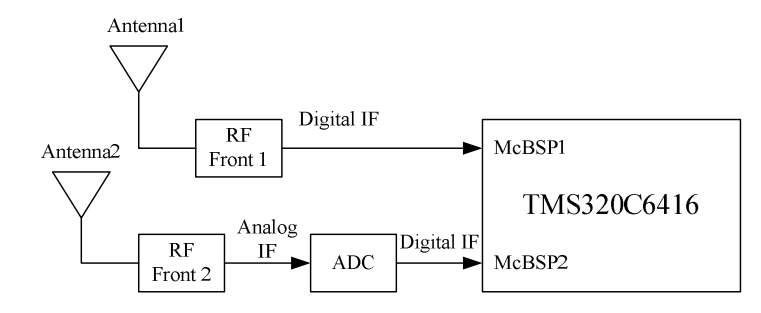
\includegraphics[width=\textwidth]{img/dsp_gnss_signal.png}
\caption{DSP GNSS Receiver Signal Input, Source:\cite{dsp_receiver}}
\label{fig:galileo_frequency_plan}
\end{figure}

Since many satellite navigation systems use similar principles, some software modules can be reused on different signal sources. For example, in GPS and Galileo, the positioning and acquisition modules are common\cite{dsp_receiver}. The software architecture proposed by \cite{dsp_receiver} contains three main tasks: tracking task, positioning task and acquisition task, in the order of task priority. Because of the multi-constellation support, two tracking tasks will run at the same level of priority. In the end we can see that the receiver proposed by the authors of \cite{dsp_receiver} can track 10 satellites in single constellation mode and 5 satellites in two constellations mode.

\subsection{MBOC Receiver\cite{ref_station_receiver}}
\label{subsec:mboc_recv}

The paper \cite{ref_station_receiver} presents the designing of a reference station receiver for Galileo and GPS. Since this receiver is designed as a reference station for the mission segment, it requires high quality measurements for pseudorange, carrier phase and status information in order to compute the errors and the integrity of navigation signal\cite{ref_station_receiver}. The work of the authors is based on their previous experience with Galileo and GNSS at Thales Alenia Space. This station is designed to work on the following signals\cite{ref_station_receiver}:

\begin{itemize}
    \item GPS L1/L2
    \item Galileo E1B, E1C, E6B, E6C, E5a, E5b, E5AltBOC
    \item Giove E1A and E6B
\end{itemize}

\begin{figure}[h]
\centering
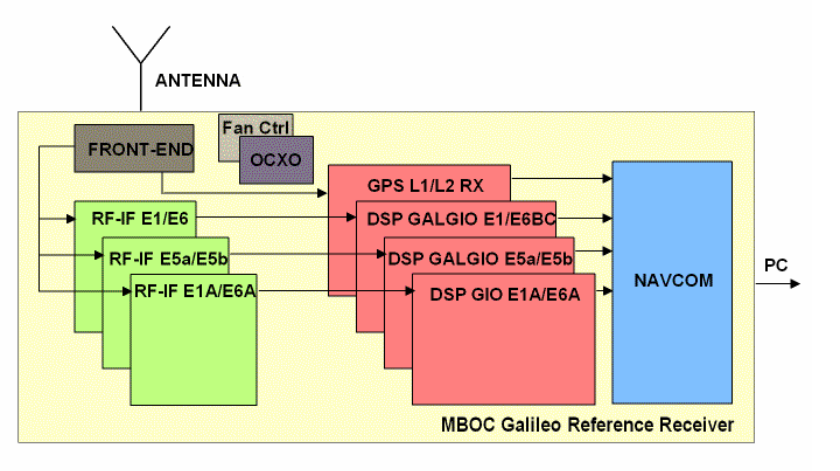
\includegraphics[width=\textwidth]{img/mboc_architecture}
\caption{MBOC Receiver Architecture, Source:\cite{ref_station_receiver}}
\label{fig:mboc_architecture}
\end{figure}

The architecture proposed by \cite{ref_station_receiver} can be seen in Figure \ref{fig:mboc_architecture}. It is composed of a high-performance multi-band active GNSS antenna with filters and low noise amplifier, RF front-end for further amplification and filtering, RF down-converters, three Digital Signal Processors and a Navigation \& Communication Processor which implements the navigation processing. 

The RF part of the system are responsible for splitting of the signal from the antenna to lines corresponding to all different carriers in the signal, feeding DC bias for the active antenna and compensating for the cable losses. The next part is the intermediate frequency down converter which also performs automatic gain control (AGC)\cite{ref_station_receiver}. 

\begin{figure}[h]
\centering
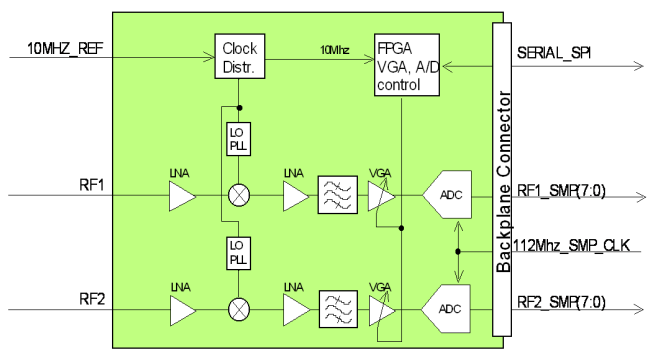
\includegraphics[width=\textwidth]{img/rf_if_block}
\caption{RF-IF Board Block Diagram, Source:\cite{ref_station_receiver}}
\label{fig:rf_if_block_diagram}
\end{figure}

The DSP Block is responsible for\cite{ref_station_receiver}:
\begin{itemize}
    \item Acquisition and tracking of signal.
    \item Measuring pseudorange, carrier phase doppler and carrier-to-noise ratio.
    \item Decoding navigation messages.
    \item performing satellite prediction and selecting satellite tracking channels based on the predictions.
    \item Managing RF-IF AGC.
\end{itemize}

The receiver channels are implemented in FPGA chips based on a Thales Alenia Space proprietary technology called GALVANI\cite{ref_station_receiver}. The signal processing chain is shared between the Galvani FPGAs and a digital signal processor. The Galvani hardware is composed of channels, also called Single Frequency Channels (SFC)\cite{ref_station_receiver} which consist in a matrix of signal processing elements. The SFC implements all the necessary modules for demodulating the GNSS signal. The Galvani cores includes\cite{ref_station_receiver}:

\begin{itemize}
    \item IF Real to Complex Converter (RCC) which takes at it's input 3 to 8 bits digitized samples and performs filtering, down-conversion to baseband, sample decimation.
    \item Code and Carrier tracking
    \item Time base generator for synchronizing with other external devices.
    \item Viterbi decoder
    \item DSP interface
\end{itemize}

\begin{figure}[h]
\centering
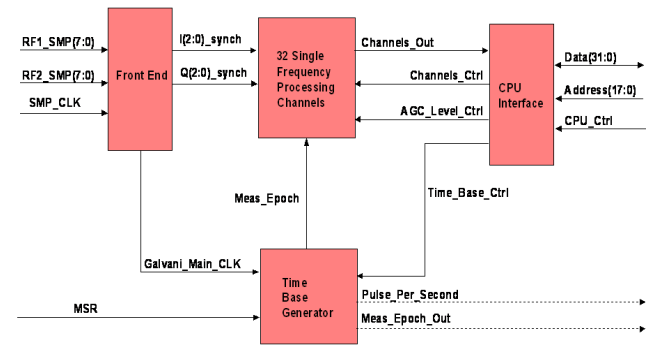
\includegraphics[width=\textwidth]{img/galvani_core}
\caption{RF-IF Board Block Diagram, Source:\cite{ref_station_receiver}}
\label{fig:galvani_core}
\end{figure}

The next component of the receiver is the Navigation and Communication Subsystem which is responsible for taking the observables processed by the DSP subsystem and computing the navigation solution and then comunicating the solution to the user, in this case it is connected to a computer \cite{ref_station_receiver}. The NavCom board is based on the Texas Instruments digital signal processor, the TMS320C6713, which is similar to the DSP model used by the authors in \cite{dsp_receiver}.

The testing performed by the authors in \cite{ref_station_receiver} shows that the reference receiver are compliant with the interference tests required for Galileo Sensor stations. In the end of the article the authors also propose a novel proprietary technique for E1 and E6 signals tracking called "Mirror rotation"\cite{ref_station_receiver}. 

\subsection{IFEN E6-B/C Receiver\cite{e6breceiver}}
\label{subsec:e6b_recv}
The authors of paper \cite{e6breceiver} present the development and testing of an E6-B/C signal GNSS receiver. This receiver is based on work done by the German company IFEN GmbH. The receiver is based on FPGA and supports multiple constellations and multiple frequencies with 50 MHz bandwidth. The receiver also incorporates two Arm Cortex A8 processors running embedded Linux \cite{e6breceiver}. The receiver support four channel high-speed ADC for signal sampling. It includes a high speed USB3 interface that can output the complex baseband signal stream to a computer. The baseband signal is the pre-processed by other FPGAs. The signal stream is then processed by software running on the Cortex A8 processors \cite{e6breceiver}.

\begin{figure}[h]
\centering
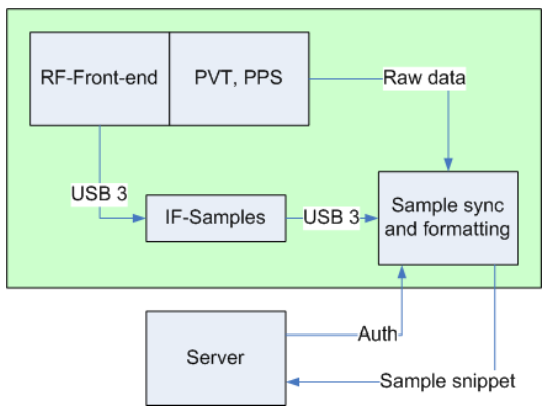
\includegraphics[scale=0.7]{img/e6b_architecture.png}
\caption{IFEN Receiver Architecture, Source:\cite{e6breceiver}}
\label{fig:e6b_architecture}
\end{figure}

The authors of \cite{e6breceiver} performed several tests in order to asses the performance of the receiver. The signal processing test result have been performed with a signal generator and the results are presented in Table \ref{table:3}. The test results using the both signal simulator and real signals are good and correspond to the theoretical expectations.

\begin{table}[h!]
\centering
\begin{tabular}{| m{12em} | m{12em} | m{12em}|}
    \hline
    Test & Description & Metric/Criteria \\
    \hline
    Multi-Signal  & Acquire and track GPS L1 and L2P, Galileo E1, E5a, E5b, E6 & All signals acquired and tracked, PVT is obtained for all signals \\
    \hline
    E6 encrypted code & Acquire and track spreading code encrypted E6 signal with key change & Tracking of encrypted signal; maintain C/N0 during key change \\
    \hline
    Signal sensitivity & Acquire and track weak signals & Tong acquisition on 34dBHz, Tracking on 28dBHz \\
    \hline
    Cold/Warm start acquisition & Measure the acquisition time & Acquisition time in line with Tong search time \\
    \hline
    Measurement Quality & Check tracking observation tracking noise vs. expectations & Tracking code range/carrier range noise in line with theory \\
    \hline
    Interference handling & Show pulse blanker and spectral filter performance & Recovery of signal when interference mitigation enabled \\
    \hline
    SAS & Test the Signal Authentication Sequences approach & Provision of correlation values when using primary code as signal sequence \\
    \hline
    RPA & Remote Processing Authentication sample collection & Check if correlation in samples is at zero code phase \\
    \hline
    
\end{tabular}
\caption{Receiver Signal Processing Tests. Source: \cite{e6breceiver}}
\label{table:3}
\end{table}